% Requirements for openETCS --- WP2
% Author: Sylvain Baro (SNCF), Jan Welte TUBs
% Version 2.0.0


\documentclass{template/openetcs_article}
% Use the option "nocc" if the document is not licensed under Creative Commons
%\documentclass[nocc]{template/openetcs_article} 
\usepackage{rotating,url,color}
\graphicspath{{./template/}{.}{./images/}}
\begin{document}
\frontmatter
\project{openETCS}

%Please do not change anything above this line
%============================
% The document metadata is defined below

%assign a report number here
\reportnum{OETCS/WP2/D2.6-9~--~2.0.0}

%define your workpackage here
\wp{Work-Package 2: ``Requirements''}

%set a title here
\title{Requirements for openETCS}

%set a subtitle here
%\subtitle{A template for short document. Adapted from report template.}

%set the date of the report here
\date{May 2013}

%define a list of authors and their affiliation here

\author{Sylvain Baro}
\affiliation{SNCF}
\author{Jan Welte}
\affiliation{TU-BS}  
  
% define the coverart
\coverart[width=350pt]{openETCS_EUPL} 

%define the type of report
\reporttype{Requirements Document}


%
% End of QA Zone
\begin{abstract}
This document provides the list of higher level requirements for the openETCS project. 
\end{abstract}

%=============================
%Do not change the next three lines
\maketitle

% 
% QA zone

\begin{tabular}{|p{4.4cm}|p{8.7cm}|}
\hline
\multicolumn{2}{|c|}{Document information} \\
\hline
Work Package &  WP2  \\
Deliverable ID or doc. ref. & D2.6-9\\
\hline
Document title & Requirements for openETCS \\
Document version & 2.0.0 \\
Document authors (org.)  & Sylvain Baro (SNCF), Jan Welte (TUBs) \\
\hline
\end{tabular}

\begin{tabular}{|p{4.4cm}|p{8.7cm}|}
\hline
\multicolumn{2}{|c|}{Review information} \\
\hline
Last version reviewed & 1.1.0 \\
\hline
Main reviewers & Marielle Petit-Doche,  Merlin Pokam, Guillaume Pottier, Uwe Steinke, Klaus-R\"udiger Hase, Bernd Hekele,
Hardi Hungar, Marc Behrens, Cyril Cornu, Fr\'ederique Vall\'ee \\
\hline
\end{tabular}

\begin{tabular}{|p{2.2cm}|p{4cm}|p{4cm}|p{2cm}|}
\hline
\multicolumn{4}{|c|}{Approbation} \\
\hline
  &  Name & Role & Date   \\
\hline  
Written by    &  Sylvain Baro & System Eng.  & \\
\hline
Approved by & Gilles Dalmas & WP2 leader & \\
\hline
\end{tabular}

\begin{tabular}{|p{2.2cm}|p{2cm}|p{3cm}|p{5cm}|}
\hline
\multicolumn{4}{|c|}{Document evolution} \\
\hline
Version &  Date & Author(s) & Justification  \\
\hline  
0.0.0 & 01/01/13 & S. Baro &  Document creation  \\
\hline  
0.1.0 & 15/01/13 & S. Baro &  Request for comment to some partners, version for review  \\
\hline  
1.0.0 & 05/03/13 & S. Baro &  Version after first review. Req. version is 1. \\
\hline
1.1.0 & 19/04/13 & S.~Baro, J.~Welte &  Update after workshop on safety and tools. Updated req. version is X.\\
\hline
2.0.0 & 31/05/13 & S.~Baro  &  Final version after review. Updated req. version is 2.\\
\hline
\end{tabular}

\newpage

\tableofcontents
%\listoffiguresandtables
\newpage





%=============================
% The actual document starts below this line
%=============================


%%%%%%%%%%%%%%%%%%%%%%%%%%%%%%%%%%%%%%%%%%%%%%%%%%%%%%%%%%%%%%
%%%              My macros (=> Sylvain Baro)               %%%
%%%%%%%%%%%%%%%%%%%%%%%%%%%%%%%%%%%%%%%%%%%%%%%%%%%%%%%%%%%%%%
\newcommand{\docend}{{\begin{center}\large\textbf{<End of Document>}\end{center}}}
\newcommand{\tbd}{\colorbox{cyan}{\%\%To Be Defined\%\%}}
\newcommand{\tbc}{\colorbox{cyan}{\%\%To Be Confirmed\%\%}}
\newcommand{\todo}[1]{\colorbox{cyan}{\%\%{#1}\%\%}}
\newlength{\origindent}

\newenvironment{issue}{
	\begin{quote}
	\begin{itshape}Open Issue. 
}{
	\end{itshape}
	\end{quote}
}

\newenvironment{comment}{
	\begin{quote}
	\begin{itshape}Comment. 
}{
	\end{itshape}
	\end{quote}
}

\newenvironment{justif}{
	\begin{quote}
	\begin{itshape}Justification. 
}{
	\end{itshape}
	\end{quote}
}
%% Requirements.


\newcounter{reqnum}
\setcounter{reqnum}{0}
\newcounter{subreqnum}
\newcounter{subsubreqnum}
\newlength{\partopbuf}
\newlength{\topbuf}

% Automated numbering versions of the macros
\newcommand{\req}[1]{\addtocounter{reqnum}{1} \setcounter{subreqnum}{0}
	\begin{description}\item[{\small\reqt-X-\thereqnum}] #1\end{description}
}

\newcommand{\subreq}[1]{
	\addtocounter{subreqnum}{1} \setcounter{subsubreqnum}{0}
	\addtolength{\leftmargini}{1cm}
	\begin{description}
	\item[\hspace{0.5cm}{\small\reqt-X-\thereqnum.\thesubreqnum}] #1
	\end{description}
	\addtolength{\leftmargini}{-1cm}
}

\newcommand{\subsubreq}[1]{
	\addtocounter{subsubreqnum}{1}
	\addtolength{\leftmargini}{2cm}
	\begin{description}
	\item[\hspace{1cm}{\small\reqt-X-\thereqnum.\thesubreqnum.\thesubsubreqnum}] #1
	\end{description}
	\addtolength{\leftmargini}{-2cm}
}

% Fixed version of the commands
\newcommand{\reqfixed}[3]{\addtocounter{reqnum}{1} \setcounter{subreqnum}{0}
	\begin{description}\item[{\small\reqt-#1-#2}] #3\end{description}
}

\newcommand{\subreqfixed}[4]{
	\addtocounter{subreqnum}{1} \setcounter{subsubreqnum}{0}
	\addtolength{\leftmargini}{1cm}
	\begin{description}
	\item[\hspace{0.5cm}{\small\reqt-#1-#2.#3}] #4
	\end{description}
	\addtolength{\leftmargini}{-1cm}	
}

\newcommand{\subsubreqfixed}[5]{
	\addtocounter{subsubreqnum}{1}
	\addtolength{\leftmargini}{2cm}
	\begin{description}
	\item[\hspace{1cm}{\small\reqt-#1-#2.#3.#4}] #5
	\end{description}
	\addtolength{\leftmargini}{-2cm}	
}

% Citation of the requirement

% Citation of the reference (for markup purpose)
%\newcommand{\refreq}[1]{\textbf{#1}}

% Citation of the reference and text (for markup purpose)
% The purpose of this is to automatically replace the placeholder by the 
% full text. \fullrefreq{R-xxx}{} or \fullrefreq{R-xxx}{blabla} 
% will be replaced by \fullrefreq{R-xxx}{text of the R-xxx requirement} 
%\newcommand{\fullrefreq}[2]{\textbf{#1}: \textrm{#2}}


\def\reqt{R-WP2/D2.6}
% Start here


\section{Introduction}
The purpose of this document is to enumerate the meta-requirements of the projects: \emph{i.e.} 
the requirements on the modelling, processes, toolchain, validation and verification. 
The purpose of this document is 
not to provide the system and safety requirements that will specify the model/software 
developed in the OpenETCS project.

The requirements found in the CENELEC standards as well as those found in the ERTMS specifications
are not rewritten here. The required plans for the 
project shall be written according to what is required in the standards (see Sect.~\ref{standards}),
then reviewed. Once this task is done, the plans will be the reference for the project.
In the meantime, one can refer to the standards, or to the D2.2 document.

The present document corresponds to the WP2 deliverables D2.6 to D2.9, with the following mapping.

\begin{tabular}{|lll|}
\hline
Deliverable & Title & Chapters \\
\hline
D2.6 & Requirements for the model & \ref{sysarchi}, \ref{models}, \ref{language} \\
\hline
D2.7 & Requirements for the API & \ref{RTMAPI} \\
\hline
D2.8 & Requirements for tools & \ref{language}, \ref{toolchain} \\
\hline
D2.9 & Requirements for V\&V & \ref{safety}, \ref{vnv}\\
\hline
\end{tabular}

\section{Reference documents}
\subsection{Standards \& ERA documents}
\label{standards}
\begin{itemize}
\item CENELEC EN 50126-1 --- 01/2000 --- \emph{Railways applications –- The specification and 
demonstration of Reliability, Availability, Maintenability and Safety (RAMS) –- Part 1: 
Basic requirements and generic process}
\item CENELEC EN 50128 --- 10/2011 --- \emph{Railway applications -- Communication, signalling and 
processing systems -- Software for railway control and protection systems}
\item CENELEC EN 50129 --- 05/2003 --- \emph{Railway applications –- Communication, signalling and 
processing systems –- Safety related electronic systems for signalling}
\item CCS TSI --- \emph{ CCS TSI for HS and CR transeuropean rail has been adopted by a Commission Decision 2012/88/EU on the 25th January 2012}
\item SUBSET-026 3.3.0 --- \emph{System Requirement Specification}
\item SUBSET-076-x (not yet released for baseline 3) --- Test related ERTMS documentation
\item SUBSET-088 (not yet released for baseline 3) --- \emph{ETCS Application Levels 1 \& 2 - Safety Analysis}
\item SUBSET-091 3.2.0 --- \emph{Safety Requirements for the Technical Interoperability
of ETCS in Levels 1 \& 2}
\end{itemize}
\subsection{Project documents}
\begin{itemize}
\item FPP --- \emph{Project Outline Full Project Proposal Annex OpenETCS} -- v2.2
\item D2.1 --- \emph{Report on existing methodologies} --- Jan Welte and Hansj\"org Manz
\item D2.2 --- \emph{Report on CENELEC standards} --- Merlin Pokam and Norbert Sch\"afer
\end{itemize}

\section{Conventions}
The requirements are prefixed by “R-zz-x-y”, and are written in a roman typeface, where ``R'' 
stands for ``Requirement'', ``zz'' identifies the source document,``x'' 
is the version number and``y'' is the identifier of the requirement. All the text 
written in italics is not a requirement: it may be a note, an open issue, an 
explanation of the requirements, or an example.

\section{Glossary}
\begin{description}
\item[API] Application Programming Interface
\item[FFM] Fully-Formal Model
\item[FME(C)A] Failure Mode Effect (and Criticity) Analysis
\item[I/O] Input/Output
\item[OBU] OnBoard Unit
\item[QA] Quality Assurance
\item[RBC] Radio Block Center
\item[RTM] RunTime Model
\item[SIL] Safety Integrity Level
\item[SFM] Semi-Formal Model
\item[SRS] System Requirement Specification (in this document, this is equivalent to the SUBSET-026 of the TSI)
\item[SSRS] SubSystem Requirement Specification
\item[THR] Tolerable Hazard Rate
\item[V\&V] Verification \& Validation
\end{description}

\section{Goals}
The following goals for the projects were considered for the writing of this document. Please note that 
they are \emph{not} listed by order of priority, but in an arbitrary order.

\subsection{Goal 1: Formalization of the SRS into a high level, simulable, semi-formal and formal model}
The first goal of the project is to propose a formalization of a subset of the on-board subsystem,
as defined in the SUBSET-026, for the chosen reference baseline. 

The purpose of the formalization is:
\begin{itemize}
\item to enhance the understanding of modelled subset;
\item to allow formal analysis of the modelled subset;
\item to be able to animate the model for testing and analyzing purpose;
\item to provide information on the completeness and soundness of the SUBSET-026;
\item to be used as a reference formal specification for the implementation of an OBU 
(by the OpenETCS project team and by industrial actors);
\item \dots
\end{itemize}

In order to conduct this formalization, a part of the tool chain and methodology defined (see Goal 2) 
will be used.

There will be two models created to satisfy this goal. One semi-formal simulable (but not in real time)
model, for which we aim to model all the requirements considered in the scope by the system design, covering as
much features as possible of the Onboard Unit.

On chosen parts of the system, this model will be completed with a strictly formal model. This will allow to improve
the understanding of the system, and will provide complementary elements for the verification and validation using formal proof. 

This will also allow to demonstrate the feasibility of the process using both semi-formal and formal modelization 
and the capabilities of analysis on the formal model using formal methods. 

\subsection{Goal 2: Definition of process/methodologies required for the safety validation
of the model}

The full safety process needed for the OpenETCS to be \emph{certifiable} according to the CENELEC standards
shall be described. The safety plan and safety case concept will detail precisely which activities 
are required or not with regard to the scope and the context of the project.

The process has in particular to ensure that toolchain, formalized SUBSET-026 specification and models are certifiable 
according to these standards while emerging from an open source environment. 

\subsection{Goal 3: Apply the safety activities on a subset of the project}
Because the full design, development, validation and safety analysis process for a SIL4 OBU
is a huge task far beyond the project possibilities, the full safety activities will not be conducted
on the whole subsystem. 

The safety analyses as described in the safety plan and safety case concept shall be conducted on a selected 
subset of the system, and on a selected subset of safety properties. It will start with system-level safety 
activities, then go down into the semi-formal, then formal model.


\subsection{Goal 4: Definition of a tool chain for developing on onboard software that can fulfill the EN 50128 
requirements}
These tools must be \emph{qualified} according to the corresponding tool level of EN 50128 (considering the 
process for which they are used), but will not be certified as part of the project.

By the combination of Goal 1, 2 and 3, it should be possible for the industry to build an ETCS 
onboard software:
\begin{itemize}
\item By using OpenETCS model\,\footnote{Or \emph{models} if several models are developed. In order to enhance readability,
I will use the singular even if it could cover a semi-formal model and a formal model.} and proving the implementation satisfies 
the model;
\item By using the OpenETCS toolchain with their own model;
\item By using the OpenETCS model and toolchain.
\end{itemize}

\subsection{Goal 5: Building a non Vital executable demonstrator/simulator of the model}
From the model, an executable software will be derived. This software will be used for simulation and 
demonstration. This software will be completely non Vital. It will be able to execute in real time and to 
interface with other components. 

\section{Project outline}
In order to pursue these goals, the development cycle for the project may be presented as follow. 

\textbf{Please note that this is just an outline of the activities, not the project plan, nor the 
Q\&A, nor the Validation plan. The \emph{verification} arrows where not represented on this outline in order 
not to clutter the drawing. Also note that the activities needed for the toolchain are not
covered here.}

\begin{figure}
  \centering
  \fbox{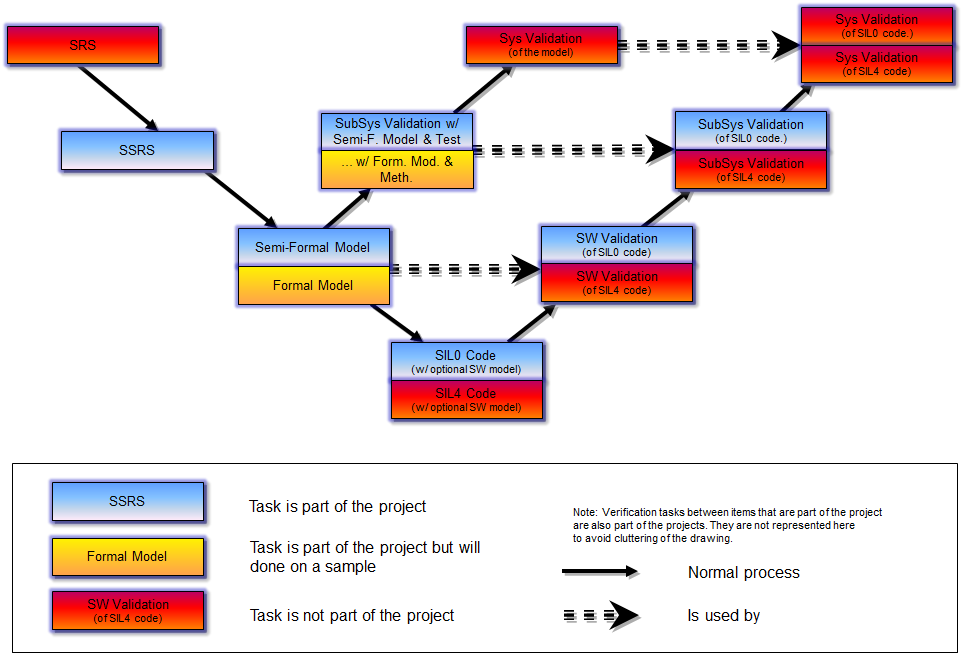
\includegraphics[scale=0.65]{Process1.png}}
  \caption{Main process}
  \label{fig:main_process}
  \centering
  \fbox{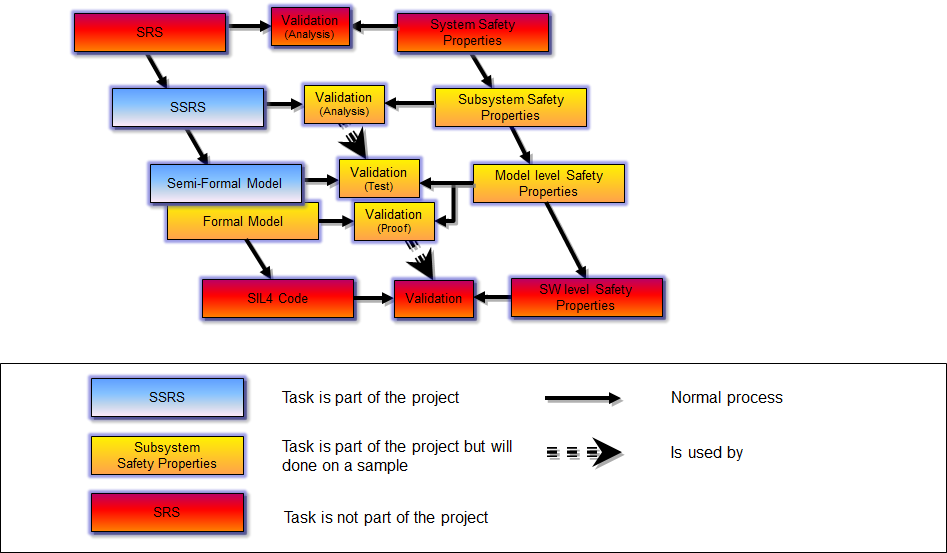
\includegraphics[scale=0.65]{Process2.png}}
  \caption{Safety analyses}
  \label{fig:safety_process}
 \end{figure}

Fig. \ref{fig:main_process} shows the main part of the development process. This process may be seen
as a ``double-V''. The smaller V corresponds to the development and validation of the high level model. 

It starts by the SRS which is not part of the project (SUBSET-026), then outlines the boundaries and 
the applicable requirements from the SUBSET-026 that will be used in the model. This outline 
is provided in the Subsystem Requirement Specification (SSRS). This document describes the subsystem that 
will be modelled. It describes the architecture of the subsystem (functions and their I/O) and the 
requirements allocated to these functions. If necessary, the requirements are rewritten in order to 
address the I/O and to correspond to the allocation. This document also provides the Vital/Non Vital 
classification of the requirements and data stream. The architecture part is described in a 
semi-formal language, and the requirements are described in natural language.

The next step is the creation of the model itself, from the SSRS. Because this model is simulable, 
it can be validated as itself, thus the first ``closing branch'' of the V. This model will be 
semi-formal, and aims to cover the full SSRS requirements. This semi-formal model will be sidekicked with 
a formal model for some of the functions of the model.

The first ``closing branch'' corresponds to the validation of the subsystem, using the semi-formal model
(with tests) and the formal model (with proof).

The second ``closing branch'' corresponds to the production of real time code capable of running on an 
onboard computer. This code shall be derived from the semi-formal model (possibly with an intermediate
SW model between). There are two possibilities for the generation of code:
\begin{itemize}
\item a \emph{demonstrator} or \emph{simulator} (no SIL associated to this item),
\item a SIL4 implementation of the model.
\end{itemize}

The SIL0 demonstrator is a deliverable of the project openETCS. On the other hand, the project toolchain and 
methodology shall be compatible with the generation of a SIL4 software, but the generation of this SW 
and the generator used for this generation are \emph{not} part of the project.

The yellow boxes correspond to activities that should be covered completely in order to produce 
a certifiable product, but of which only a subset will be conducted in order to demonstrate the 
capabilities of the product. We consider that doing the full set of activities for the project to 
be fully compliant to CENELEC standards (\emph{i.e.} to be certifiable) is a huge task. Hence we 
should isolate a subset of this tasks, as complete in terms of tasks as possible in order to be 
convinced of the feasibility of the whole activities. 

Therefore we have to discriminate three kinds of tasks:
\begin{description}
\item[blue:] the tasks that will be completely achieved in the scope of the OpenETCS project;
\item[red:] the tasks that will be not be achieved, because they are out of the scope of the OpenETCS project;
\item[yellow:] the tasks for which a sample will be achieved, because they are in the scope of the 
OpenETCS but doing them completely is unrealistic considering the resources of the project.
\end{description}


Fig. \ref{fig:safety_process} shows activities that are needed for the safety analyses. It should 
be considered in parallel of the descending branch of the V, but has been put on a separate diagram for
the sake of clarity. These activities will be conducted on a subset of the model.
The validation tasks correspond to the safety validation of the model w.r.t. 
the safety properties.

A subset of high level safety properties are provided, 
which must be refined side-to-side with each step on the 
descending branch of the V. These properties are then used for the safety analysis of the model subset.

\section{Requirements}
\subsection{Runtime Model \& API}
\label{RTMAPI}
The framework needs to provide a list of properties and functions. If we take the parallel of the Java environment, 
some of these properties/functions will be provided by the \emph{abstract machine} properties, and some of them will 
be provided by the API.

If we consider for example ``allocation of memory'', in Java usually it is just provided by the creation of an object 
(thus in the ``Runtime model''). In C it is given by the \emph{malloc} function, which is part of the API (of course, 
we will find eventually that it leads to the runtime model too, but in the user point of view, it is
definitely part of the API).

What is considered is that at requirement level, it is not useful to know which property will come from API and which will 
come from the runtime model. It is only interesting to provide the properties themselves.

In order to avoid ambiguities, we will define the following.
\begin{description}
\item[Runtime model.] This is the abstract layer required to ``run'' the formal model. It shall provide
in the formalism part or all of the following (but not restricted to):
\begin{itemize}
\item memory management,
\item execution of state machines (or of the chosen formal objects), 
\item failures, 
\item communication between processes and concurrence,
\item \emph{real time} clock.
\end{itemize}
All these can be provided with or without safety properties. This corresponds in fact to the services 
provided by the ``abstract machine(s)'' which runs the models.
\item[API.]
 This is the functions/primitives required to complete the \emph{Runtime model}. It shall provide
the remaining of the features listed hereabove which are not provided by the Runtime model.

All these can be provided with or without safety properties.
\item[RTM/API.]
This corresponds to the Runtime Model \emph{plus} API. Therefore it should provide all the services
needed to emulate at abstract level the hardware platform that could run the software.
\item[Functional Architecture.] This corresponds to the functional boundaries between the ETCS KERNEL 
and the other functional components (JRU, DMI, Odometry, Eurobalise, Euroradio\dots). These boundaries
are described in the FIS or FFFIS. It also includes the parting of the KERNEL into different 
functions.
\end{description}

In the following requirements, we will not discriminate what is required from the API and from the 
RTM. This is the definition of these components that will allocate the requirements to the different 
parts. Hence we will only state requirements on the RTM/API.



\reqfixed{02}{043}{The RTM/API model shall provide an abstraction layer of the hardware architecture.}
\subreqfixed{02}{043}{01}{The RTM/API shall abstract memory management.}
\subreqfixed{02}{043}{02}{The RTM/API shall abstact the execution of states machine.}
\subreqfixed{02}{043}{03}{The RTM/API shall allow communication and concurrence (if requested by the model formalism).}
\subreqfixed{02}{043}{04}{The RTM/API shall allow read/write to a persistent data store.}
\subreqfixed{02}{043}{05}{The RTM/API shall allow to state \emph{real time} constraints.}
\subreqfixed{02}{043}{06}{The RTM/API shall provide emulation for a \emph{real time} clock.}

\reqfixed{01}{004}{The RTM/API shall make possible to refine the software into final code able to run 
on hardware complying the EN 50129 standard for the requested SIL.}

\reqfixed{01}{005}{The RTM/API shall allow discriminating Vital processing, data and I/O from Non Vital processing, data and I/O.}
\reqfixed{01}{006}{The RTM/API shall provide a way of communication between Vital processes and Non Vital processes.}

\begin{justif}
The purpose of these requirements is to be able to discriminate the safety part from the non 
safety part. It should be made possible to have it run on a proprietary architecture with both 
software on the same computer (with for example 2oo3, or coded monoprocessor) or on two 
different computers. One way of doing this, for example is to have some critical state 
machines with their data on one side, and the non critical part on the other side, with 
API channels to make them communicate.
\end{justif}

\reqfixed{01}{007}{The RTM/API shall allow fault injection.}
\reqfixed{01}{008}{The RTM/API shall allow logging and tracing.}
\reqfixed{01}{009}{The RTM/API shall provide a way of reading configuration data (\emph{e.g.} constants,\dots)}

\reqfixed{01}{010}{The RTM/API shall provide an abstraction layer of the communication and interfaces 
with other components.}
\begin{justif}
Even if the FIS or FFFIS requires a specific protocol (\emph{e.g.} Profibus), this protocol will not 
be implemented in the high level model. It will be considered that low level communication issues are
taken into account (= emulated) by the RTM/API.
\end{justif}



\subsection{System and Architecture}
\label{sysarchi}
\reqfixed{02}{044}{The reference ETCS baseline shall be modified only by project decision.}

\reqfixed{02}{045}{The SRS (SUBSET-026 for the reference baseline) shall be refined into a SSRS.}
\subreqfixed{02}{045}{01}{The SSRS shall identify all functions, interfaces and parameters in addition to the ones covered by the SRS but 
which are requested at functional level in order to be compliant to the SRS.}
\subreqfixed{02}{045}{02}{The SSRS shall provide a functional architecture of the OBU.}
\subsubreqfixed{02}{045}{02}{01}{The SSRS shall split the KERNEL into independent functions.}
\subsubreqfixed{02}{045}{02}{02}{The description of the architecture shall be semi-formal.}
\subsubreqfixed{02}{045}{02}{03}{This architecture shall provide the functions and the data streams between them.}
\subsubreqfixed{02}{045}{02}{04}{The SSRS shall describe which part of this architecture will be modelled.}
\subsubreqfixed{02}{045}{02}{05}{The SSRS shall provide the interfaces between the considered subsystem and its environment.}
\subsubreqfixed{02}{045}{02}{06}{When the boundary of the formalized subsystem corresponds to a FIS or FFFIS, the SSRS shall try to comply to it even when it is not mandatory.}

\subreqfixed{02}{045}{03}{The SSRS shall allocate the requirements of the SRS to the functions and their I/O.}
\subreqfixed{02}{045}{04}{The SSRS shall be compliant or shall allow compliance to the mandatory requirements from the other subsets of the TSI.}
\subreqfixed{02}{045}{05}{Traceability between the SRS and SSRS shall be provided.}
\subsubreqfixed{02}{045}{05}{01}{All interpretations, additions, refinement, omissions and design choices during the allocation have to be documented in one log and justified.}
\subsubreqfixed{02}{045}{05}{02}{The requirements allocated to other subsystemes (\emph{e.g.} RBC) shall be tracked.}

\subreqfixed{02}{045}{06}{In case of divergence between an identified national behavior and the SRS behavior, it shall be discussed and decided whether or not
the national behaviors are required in the SSRS.}
\subsubreqfixed{02}{045}{06}{01}{If it is the case, it shall be traced explicitly.}
\subsubreqfixed{02}{045}{06}{02}{If it is the case, it shall be possible by configuration to enforce pure compliance to the SRS.}

\reqfixed{02}{046}{The SSRS shall identify the Vital and Non Vital functions, requirements, and data streams.}

\subsection{Model(s)}
\label{models}
\reqfixed{02}{047}{The subsystem described in the SSRS shall be modelled into a Semi-Formal Model (SFM).}
\subreqfixed{02}{047}{01}{The SFM shall be modelled in a semi-formal means of decription.}
\subreqfixed{02}{047}{02}{The SFM shall be as consistent as possible with the SSRS level of abstraction.}
\subsubreqfixed{02}{047}{02}{01}{All the requirements of the SSRS shall be covered by the SFM.}
\subsubreqfixed{02}{047}{02}{02}{All safety requirements derived from the Hazard Log and allocated to the sub-system functionality shall be covered by the SFM}
\subsubreqfixed{02}{047}{02}{03}{Needed interpretations, refinement, additions and omissions shall be tracked and justified.}
\subsubreqfixed{02}{047}{02}{04}{If a deviation is needed, it shall be tracked and justified, and it will also be insulated as much as possible using 
proper modularity.}
\subsubreqfixed{02}{047}{02}{05}{Traceability between the SSRS and the SFM shall be provided.}
\subsubreqfixed{02}{047}{02}{06}{Exported requirements shall be tracked.}
\subsubreqfixed{02}{047}{02}{07}{Lower level safety properties refined from higher level safety properties shall be tracked.}

\reqfixed{02}{048}{The SFM design and level of description shall be simulable.}

\reqfixed{02}{049}{Some parts of the subsystem described in the SSRS shall be modelled into a Fully Formal Model (FFM).}
\subreqfixed{02}{049}{01}{The FFM shall be modelled in a strictly formal mean of description\,\footnote{Nevertheless, we will use the 
wording ``Fully Formal Model'' in order to be allowed to use a different abbreviation than for ``Semi-Formal Model''.}.}
\subreqfixed{02}{049}{02}{The FFM shall be modelled based on the SFM.}
\subreqfixed{02}{049}{03}{Traceability between the SFM and the FFM.}
\subsubreqfixed{02}{049}{03}{01}{Needed interpretations, design choices, refinement, additions and omissions shall be tracked and justified.}
\subreqfixed{02}{049}{04}{The SFM shall be designed in order to make possible the modelling and the validation of the FFM.}
\subreqfixed{02}{049}{05}{The transformation of the SFM into the FFM shall be as straightforward and automated as possible\,\footnote{%
Please note that the requirements on the FFM do not forbid a complete automation of the transformation, nor the identity
of the FFM and SFM.}.}

\reqfixed{02}{050}{The SFM design shall be modular and extensible.}
\reqfixed{02}{051}{The FFM design shall be modular and extensible.}
\subreqfixed{02}{051}{01}{The modular design of the FFM should represent a refinement of the modular SFM design.}

\reqfixed{02}{052}{Safety relevant function should be as much as possible insulated from Non Safety relevant functions.}

\subsection{Safety}
\label{safety}
Side to side with the models (SFM and FFM), should lay a set of  
static safety properties on the model. The higher level properties will be provided 
by the SUBSET-088 and SUBSET-091 documents, that we will consider here as a preliminary hazard analysis, 
because it provides us the higher level feared events.

These feared events will be refined during a Sub System Hazard Analysis (SSHA) into events of the abstraction level of the sub system, 
which will be collected in the Hazard Log. For all hazardous events named in the Hazard Log a risk analysis will be performed.
Based on the analyses suitable risk control activities a determined and collected in the Hazard Log. All hazards and their 
control activities are then refined into safety requirements/ properties\,\footnote{The document ``Safety properties for 
OpenETCS through two examples'' provides a proposal on this subject.
\url{https://github.com/openETCS/requirements/tree/master/WorkDocuments/SafetyRequirementsExamples}} which are transferred 
to the respective backlogs for the different models and their verification and validation.
The lower level Safety Properties/Feared Events shall address variables, state and interfaces used in the formal model.

As much as possible, formal proof would then be used to prove that the OpenETCS model never enter a Feared State, 
as long as the other subsystem (RBC, communication layer\dots) fulfill their own safety properties 
(axiom describing the environment). The exact process shall be described in the Safety Plan.
 


\reqfixed{02}{053}{A Safety Case Concept and Safety Plan shall be issued describing the safety activities for all the steps from the 
SRS to the SSRS, then to the SFM, the FFM and the source code, according to CENELEC EN~50126, EN~50128 and EN~50129.}
\subreqfixed{02}{053}{01}{All the output documents required by the EN~50126, EN~50128 and EN~50129 for 
each step of the lifecycle shall be described, or their lack shall be justified.}


\reqfixed{02}{054}{The safety activities shall at least be applied on a sample of the on-board functionalities and the respective safety 
requirements to demonstrated the suitability of the safety plan.}

\reqfixed{02}{055}{The safety activities shall aim at a THR compatible with the SUBSET-091.}

\reqfixed{02}{056}{The safety analysis shall consider as higher level Feared Events the events named in the SUBSET-091 in respect to the  
 scope of the subsystem.}
\subreqfixed{02}{056}{01}{Those Feared Events shall be refined to SRS and SSRS levels, then to the model level, and allocated to the functions to 
determine hazardous events.}
\subreqfixed{02}{056}{02}{The refinement shall only be done for a sample part of the system.}

\reqfixed{02}{057}{The model-level safety requirements shall be written in the same degree of formality as the corresponding model or higher.}


\reqfixed{02}{058}{It shall be verified that the SFM, FFM and source code complies with all respective safety requirements:}
\subreqfixed{02}{058}{01}{either by a real-time constraint\,\footnote{This real-time constraint is not guaranteed in the model itself, but can be expressed in the model using the RTM/API.};}
\subreqfixed{02}{058}{02}{using test for the SFM;}
\subreqfixed{02}{058}{03}{using formal proof for the part modelled in the FFM and for the sorce code;}
\subreqfixed{02}{058}{04}{if a safety requirement/property can not be proven, testing covering all reasonable possible events shall be used.}

\reqfixed{02}{059}{The software safety activities will comply to the requirements of CENELEC 50128.}
\reqfixed{02}{060}{The model safety activities will be adapted from the requirements of CENELEC 50128.}

\subsection{Verification and Validation}
\label{vnv}
The already provided requirements require a safety plan compliant to the CENELEC EN~50126, 50128 and 50129.
This pulls a number of requirements on V\&V, including Verification and Validation plans. On the topic of 
compliance to EN~50128, one shall also refer to the D2.2 document.


\reqfixed{02}{061}{A Verification plan shall be issued and complied with.}
\subreqfixed{02}{061}{01}{The verification plan shall provide a method to demonstrate the requirements covering all the development artifacts.}
\subreqfixed{02}{061}{02}{The verification plan shall state all verification activities required for each of these development artifacts.}
\reqfixed{02}{062}{A Validation Plan shall be issued and complied with.}
\subreqfixed{02}{062}{01}{The validation plan shall provide a method to validate all functional and safety requirements over all development artifacts.}
\subreqfixed{02}{062}{02}{The validation plan shall state all validation activities required for each of these development artifacts.}

\reqfixed{01}{021}{The test plan shall comply the mandatory documents of the SUBSET-076, restricted to the scope of 
the OpenETCS project.}
\begin{justif}
It will possibly be difficult to model all the tests in the course of the project, but the test plan should at least 
be complete.
\end{justif}


\reqfixed{02}{063}{Each design artifact needs a reference artifact which it implements (\emph{e.g.} code to detailed model, SFM to SSRS model\dots)}
\subreqfixed{02}{063}{01}{The implementation between them relation shall be specified in detail.}
e.g. for state machine and a higher level state machine mapping of interfaces, states and transition is required.
This includes additional invariants, input assumptions and further restrictions. This informaiton is the basis for verification activities.
\subreqfixed{02}{063}{02}{The design of the artifacts shall be made such to allow verifiability as far as possible.}
\reqfixed{02}{064}{The findings from the verification shall be traced, and will be adequately addressed (taken into consideration, or postponed or discarded with a justification).}




\subsection{Language and formalism}
\label{language}
\reqfixed{02}{065}{The description of the SFM shall be understandable by domain experts with a reasonable amount of specific training.}
\subreqfixed{02}{065}{01}{The means of description of the SFM  shall provide simple graphical representation for component relations, 
data-flow and system behavior (which cover process sequence and state evolution).}
\subreqfixed{02}{065}{02}{The means of description of the SFM  shall provide visual simulation of the system behavior.}

\reqfixed{02}{066}{The means of discription used to formalize safety properties shall be formal and declarative.}
\subreqfixed{02}{066}{01}{The formalism shall be understandable by domain experts without specific training.}
\subreqfixed{02}{066}{02}{The formalism shall be able to state:}
\subsubreqfixed{02}{066}{02}{01}{logical statements,}
\subsubreqfixed{02}{066}{02}{02}{time constraints.}

\reqfixed{02}{067}{All means of description used shall be standardized or at least documented in detailed.}
\reqfixed{02}{068}{The means of descriptions used for SSRS, SFM and FFM modeling shall be open for the use with different tool \emph{via}:}
\subreqfixed{02}{068}{01}{direct exchange of the model data file;}
\subreqfixed{02}{068}{02}{or fully automated translation of the model data file.}
 

\reqfixed{02}{069}{The means of description for the SFM shall be able to formalize:}
\subreqfixed{02}{069}{01}{State machines,}
\subreqfixed{02}{069}{02}{Time-outs,}
\subreqfixed{02}{069}{03}{Truth tables,}
\subreqfixed{02}{069}{04}{Arithmetics,}
\subreqfixed{02}{069}{05}{Braking curves,}
\subreqfixed{02}{069}{06}{Logical statements,}
\subreqfixed{02}{069}{07}{Messages and fields.}


\reqfixed{02}{070}{The language for the FFM shall be able to formalize as much as possible of:}
\subreqfixed{02}{070}{01}{State machines,}
\subreqfixed{02}{070}{02}{Time-outs,}
\subreqfixed{02}{070}{03}{Truth tables,}
\subreqfixed{02}{070}{04}{Arithmetics,}
\subreqfixed{02}{070}{05}{Braking curves,}
\subreqfixed{02}{070}{06}{Logical statements,}
\subreqfixed{02}{070}{07}{Messages and fields.}


\begin{comment}
These requirements do not state that all these objects need to be \emph{first order objects} of
the language. They only state that it should be possible to formalize and manipulate them.

It is to be noted that if (for example) braking curves are objects of the language, it shall be
proved that they are sound, and that the code generation for these objects is also sound.
\end{comment}

\reqfixed{02}{071}{The mean of description of the SFM shall allow it to be simulable.}

\begin{comment}
This requirement is in the section ``language and formalism'' because in order for the model to 
be simulable, it has to be able to yield some algorithmic content and determinism (or a way 
of determining a non-deterministic model), which is indeed a property on the formal aspects
of the model. In the other hand, it is also a requirement on the tool chain, hence there are also
some requirements on this topic in Sect.~\ref{toolchain}.
\end{comment}

\reqfixed{02}{072}{It shall be possible to assert logical properties on the SFM and FFM (\emph{e.g.} invariants).}
\subreqfixed{02}{072}{01}{It shall be possible to check the conformance of these properties at runtime on the SFM.}
\subreqfixed{02}{072}{02}{It shall be possible to prove the conformance of the FFM to these properties.}

\reqfixed{02}{073}{The language and formalism should be extensible.}


\subsection{Tools chain}
\label{toolchain}
\subsubsection{Usage}

\reqfixed{02}{074}{The tools chain shall be composed as far as possible of Open Source components licensed under a license compatible with the EUPL license.}
\subreqfixed{02}{074}{01}{Closed source components may be used, but only if their use is not mandatory in the process, 
or if an open source counterpart is provided.}
\subreqfixed{02}{074}{02}{If a closed source component is used, it has to be displayed how an open source component has to be designed to replace the closed component later.}

\reqfixed{02}{075}{The tools chain shall be portable to common operating systems.}
\subreqfixed{02}{075}{01}{The tool chain shall run stable on all main operating systems.}
\subreqfixed{02}{075}{02}{The tool chain shall run with a good performance on all main operating systems.}
\subreqfixed{02}{075}{03}{The tool chain shall run on at least one major open source operating system.}

\reqfixed{02}{076}{The tools used in the tool chain shall be able to cooperate, \emph{i.e.} the outputs of one 
tool will be suitable to be used as the inputs of another tool.}
\subreqfixed{02}{076}{01}{All possible input and output formats of a tool have to be documented.}
\subreqfixed{02}{076}{02}{Open data formats shall be used for data exchange.}


\reqfixed{01}{032}{If tools are required for configuration management, they will be considered as part of the tool chain.}

\reqfixed{02}{077}{The tools chain shall allow to generate executable code from the model(s).}

\subsubsection{Information management}
\reqfixed{02}{078}{The tools chain shall be sufficiently robust to allow large software management (at least covering the scope as identified by the SSRS).}
\subreqfixed{02}{078}{01}{It shall allow modularity at any level (proof, models, software).}
\subreqfixed{02}{078}{02}{It shall allow the management of documentation.}
\subreqfixed{02}{078}{03}{It shall allow distributed software development.}
\subreqfixed{02}{078}{04}{It shall allow simultaneous multi user usage.}
\subreqfixed{02}{078}{05}{It shall include an \emph{issue-tracking system}, in order to allow change management and 
errors/bugs management.}
\subreqfixed{02}{078}{06}{It shall allow to document/track the differences between the models and the ERTMS reference.}
\subreqfixed{02}{078}{07}{It shall support management of subsequent Subset-026 versions, as well as differences tracking between Subset-026 versions.}
\subreqfixed{02}{078}{08}{It shall allow concurrent version development, or be compatible with tools allowing
concurrent version development.}
\subreqfixed{02}{078}{09}{The version management tools shall use model-based version control instead of text-based version control, when appropriate.}
\subreqfixed{02}{078}{10}{In particular it shall allow to track the roles and responsibilities of each  participant on a configuration item, at each step of the project lifecycle.}
\subreqfixed{02}{078}{11}{In particular, version management shall allow to track version of the safety properties 
together with the models.}


\reqfixed{02}{079}{The tool chain shall allow traceability between:}
\subreqfixed{02}{079}{01}{the documentation/requirements and the models,}
\subreqfixed{02}{079}{02}{the documentation/requirements and the tests,}
\subreqfixed{02}{079}{03}{the models and the tests,}
\subreqfixed{02}{079}{04}{each required level of implementation and the lower level (\emph{e.g.} higher level model \emph{vs} lower level model, 
lower level model \emph{vs} source code\dots),}
\subreqfixed{02}{079}{05}{the documentation/requirements and the models,}
\subreqfixed{02}{079}{06}{the documentation/requirements and the safety properties/requirements,}
\subreqfixed{02}{079}{07}{the models and the safety properties/requirements,}
\subreqfixed{02}{079}{08}{the tests and the safety properties/requirements.}

\subsubsection{Testing}
\reqfixed{01}{036}{The SFM shall be simulable in debug mode (step-by-step), allowing
inspection of states, variables and I/O.}
\reqfixed{01}{037}{The environment shall be emulated by high level construction of the inputs.}
\begin{justif}
``High level'' means that it will not be necessary to define bitwise the inputs at each cycle.
On the contrary, some automation will be available to define the behavior of the inputs.
\end{justif}

\reqfixed{02}{080}{The environment shall be emulated by construction of the inputs compliant to SUBSET-026.}
\reqfixed{02}{081}{The tool chain shall allow time-based test cases.}

\reqfixed{01}{038}{The tool chain shall allow to write, execute and store \emph{test cases} and \emph{use cases}
for the SFM.}
\reqfixed{02}{082}{Version management will allow to map test cases version to the SFM, the FFM and source code versions.}
\reqfixed{02}{083}{The tool chain shall allow to generate test cases for the SFM, the FFM and source code from a \emph{test model}.}
\subreqfixed{02}{083}{01}{The \emph{test model} is independant from the tested model.}
\begin{justif}
The test model can be either a model of the environment, or a model of the same subsystem that is being tested, but in both cases
this test model must be completely independant from the tested model.
\end{justif}

\reqfixed{02}{084}{The tool chain shall allow to write, execute and store test sequences combining multiple test cases for the SFM, the FFM and source code.}

\subsubsection{Conformance to standards}

\reqfixed{02}{085}{Each tool in the tool chain shall be classified among T1, T2 and T3 depending on its usage in the process.}
\reqfixed{01}{042}{The tool chain shall conform to EN~50128 requirements, for the corresponding SIL and tool 
class\,\footnote{Refer in particular to D2.2.}.}
\subreqfixed{01}{042}{01}{For T2 and T3 tools\,\footnote{T2: Tools contributing to the test or verification of the code 
or design 
\emph{e.g.} static analyzers, test generators\dots)\\ T3: tools contributing directly or indirectly
to the final code or data (\emph{e.g.} compilers, code translator\dots)}, the choice of tools shall be 
justified, and the justification shall
include how the tool's failures are covered, avoided or taken into account (ref. to EN 50128 6.7.4.2).}

\subreqfixed{01}{042}{02}{All T2 and T3 tools must be provided with their user manuals.}

\subreqfixed{01}{042}{03}{For all T3 tool, the proof of correctness  or the measure taken to guarantee the correctness 
of the output w.r.t. their specification and the inputs shall be provided.}
\subsubreqfixed{01}{042}{03}{01}{\dots for data transformation,}
\subsubreqfixed{01}{042}{03}{02}{\dots for software transformation (\emph{e.g.} translation, compilation\dots).}

\subsection{Demonstrator}
\reqfixed{02}{086}{A demonstrator software will be built from the SFM.}
\reqfixed{02}{087}{The demonstrator shall be non vital.}
\reqfixed{02}{088}{The demonstrator shall be able to run in real time.}
\reqfixed{02}{089}{The demonstrator shall comply to the standardized interfaces in order to be able to interface with other subsystems.}
\reqfixed{02}{090}{The demonstrator shall be able to run on an onboard computer.}

\docend

\end{document}
\end{document}
%LAST REQ USED = 90 % DO NOT MODIFY THIS LINE